\documentclass[letterpaper,11pt]{article}
\oddsidemargin -1.0cm \textwidth 17.5cm

\usepackage[utf8]{inputenc}
\usepackage[activeacute,spanish, es-lcroman]{babel}
\decimalpoint
\usepackage{amsfonts,setspace}
\usepackage{amsmath}
\usepackage{amssymb, amsmath, amsthm}
\usepackage{comment}
\usepackage{float}
\usepackage{amssymb}
\usepackage{dsfont}
\usepackage{anysize}
\usepackage{multicol}
\usepackage{enumerate}
\usepackage{graphicx}
\usepackage[left=1.5cm,top=2cm,right=1.5cm, bottom=1.7cm]{geometry}
\setlength\headheight{1.5em} 
\usepackage{fancyhdr}
\usepackage{multicol}
\usepackage{hyperref}
\usepackage{wrapfig}
\usepackage{subcaption}
\usepackage{siunitx}
\usepackage{cancel}
\usepackage{mdwlist}
\usepackage{svg}
\pagestyle{fancy}
\fancyhf{}
\renewcommand{\labelenumi}{\normalsize\bfseries P\arabic{enumi}.}
\renewcommand{\labelenumii}{\normalsize\bfseries (\alph{enumii})}
\renewcommand{\labelenumiii}{\normalsize\bfseries \roman{enumiii})}


\begin{document}

\fancyhead[L]{\itshape{Facultad de Ciencias F\'isicas y Matem\'aticas}}
\fancyhead[R]{\itshape{Universidad de Chile}}
\rfoot[]{pág. \thepage}

\begin{minipage}{11.5cm}
    \begin{flushleft}
        \hspace*{-0.6cm}\textbf{FI1100 Introducción a la Física Moderna}\\
        \hspace*{-0.6cm}\textbf{Tutor:} Alejandro Cartes
    \end{flushleft}
\end{minipage}

\begin{picture}(2,3)
    \put(366, -10){
\includegraphics[scale=0.9]{Imágenes/logo/dfi-fcfm.pdf}}
\end{picture}

\begin{center}
	\LARGE\textbf{Tutoría C2}\\
	\Large{Ondas acústicas, Óptica Geométrica y Ondulatoria}
\end{center}

\vspace{-1cm}
\begin{enumerate}\setlength{\itemsep}{0.4cm}

\item[]

\item Al lugar de un incendio acuden por la misma carretera rectilínea, en el mismo sentido, un coche de bomberos a una velocidad $v_b$ y una ambulancia a $v_a$. Ambos coches emiten una sirena con frecuencia $f_0$. Una persona se encuentra en el costado de la carretera a una distancia $d$ del lugar del incendio escuchando las sirenas.

\begin{enumerate}
    \item En un momento dado el coche de bomberos se encuentra a una distancia $L_b$ y la ambulancia a $L_a$ del lugar del incendio, con $L_b > L_a > d$. Para la persona ubicada en la carretera, ¿cuál de los dos sonidos emitidos en ese instante llega antes?, ¿qué sirena suena más aguda?, ¿cuál es la frecuencia de la señal que oye esa persona?

    \item Para los conductores de la ambulancia y coche de bomberos, ¿cuál es la frecuencia que le llega del otro vehículo cuando se encuentran en la posición del apartado anterior?

    \item Cuando ha transcurrido un tiempo $T$, ambos vehículos hacen sonar sus sirenas otra vez. Si en esta situación se cumple que la ambulancia está a una distancia $L_a'$ y el carro de bomberos a una distancia $L_b'$ del lugar del incendio, tal que $d>L_a'> L_b'$, ¿cómo quedan los resultados de los dos apartados anteriores?
\end{enumerate}

% \item 
%     \textbf{[P3-C1 2023-1]} Un diapasón es una varilla metálica en forma de U. El sonido emitido por el diapasón contiene una sola frecuencia que viene grabada en este dispositivo y es igual a $\SI{384}{\Hz}$. El diapasón puede usarse para poder encontrar la velocidad del sonido en una columna de aire  para esto, se busca la frecuencia en la que se produce resonancia (cuando la frecuencia del diapasón coincide con algún modo normal de la columna de aire). Considere el esquema mostrado en la figura, en donde se tiene una columna de aire en un tuvo d vidrio con un extremo abierto en la parte superior y cerrado en el otro lado mediante un pistón móvil. Cuando el pistón está a $\SI{22.8}{\cm}$ del extremo abierto se escucha resonando y, una vez más, cuando está a $\SI{68.3}{\cm}$ del extremo abierto.
% \begin{multicols}{2}
%     \begin{enumerate}
%         \item ¿Qué rapidez de sonido se implica con estos t?
%         \item ¿A qué distancia $L$ del extremo abierto estará el pistón cuando se escuche la siguiente resonancia?
%     \end{enumerate}
%     \columnbreak
%     \begin{figure}[H]
%         \centering
%         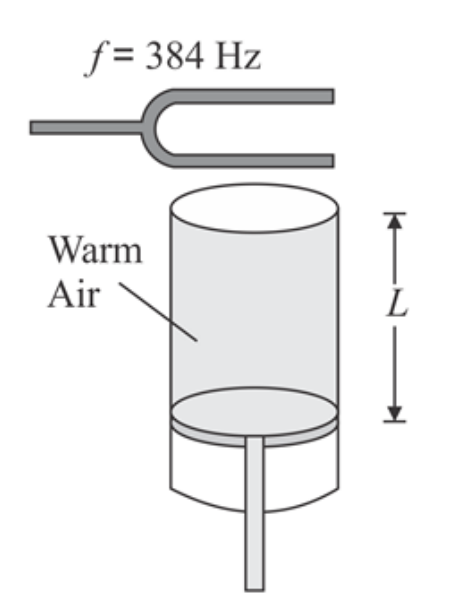
\includegraphics[width=0.4\linewidth]{Imágenes/tutorias/image.png}
%     \end{figure}
% \end{multicols}

\item 
\begin{multicols}{2}
    Se producen imágenes de un objeto sobre una pantalla usando un lente delgado convergente. Con la posición del objeto y de la pantalla fija, se mueve el lente, encontrando que la imagen se enfoca en dos posiciones distintas (como se muestra en la figura). Si las alturas de las imágenes están dadas por $h_1$ y $h_2$, respectivamente. ¿Cuál es la altura del objeto?

    \columnbreak
    
    \begin{figure}[H]
        \centering
        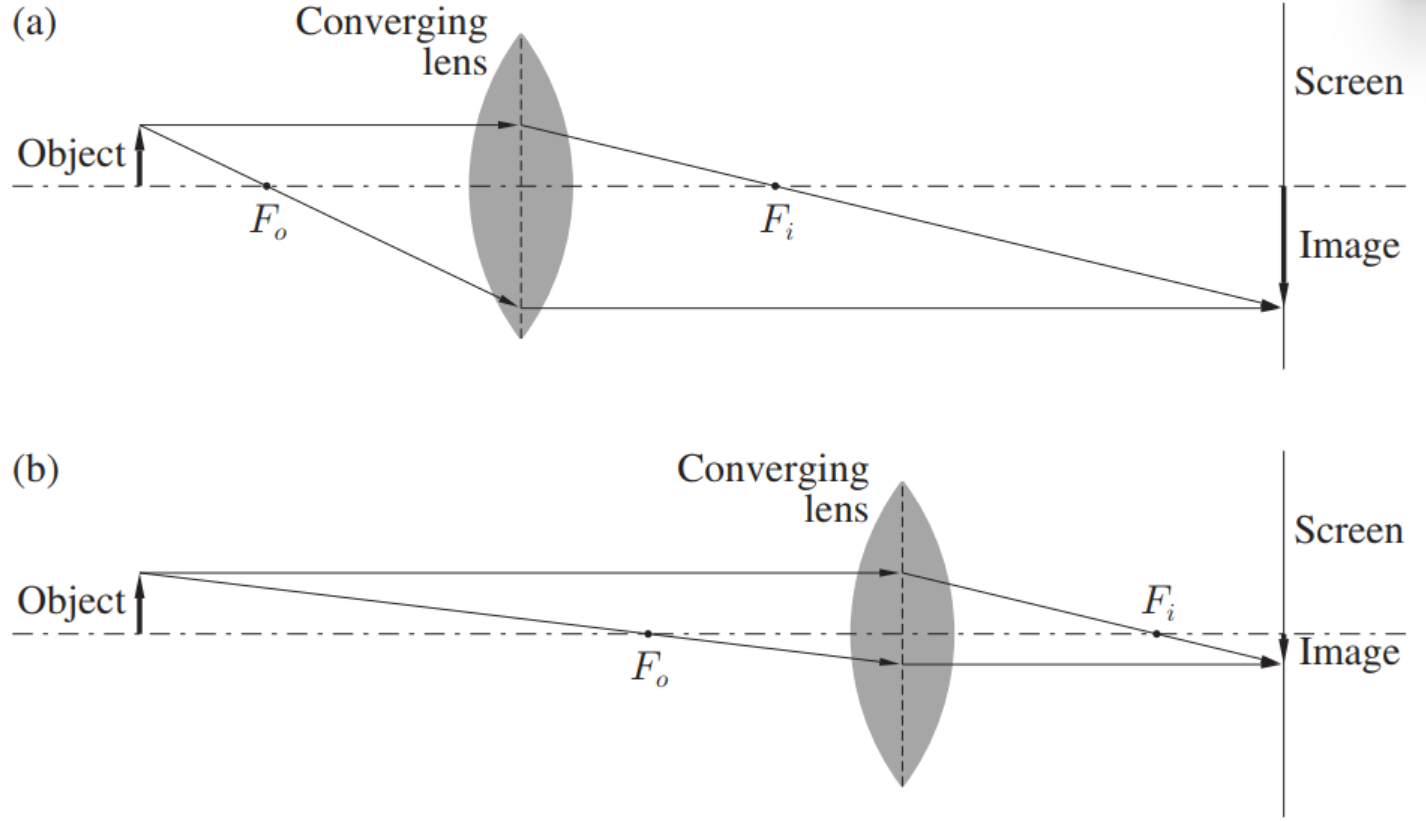
\includegraphics[width=0.7\linewidth]{Imágenes/clases/lens pos.png}
    \end{figure}
\end{multicols}

\item 
\begin{multicols}{2}
    Considere un sistema óptico compuesto por una lente convexa con longitud focal $f_L=\SI{0.02}{\m}$ y un espejo convexo $M$ de radio $R_M=\SI{0.12}{\m}$. Si la distancia entre el lente y el espejo es $d=\SI{0.04}{\m}$, determine la ubicación de la imagen de un objeto ubicado a $\SI{0.03}{\m}$ de la lente

    \columnbreak
    \begin{figure}[H]
        \centering
        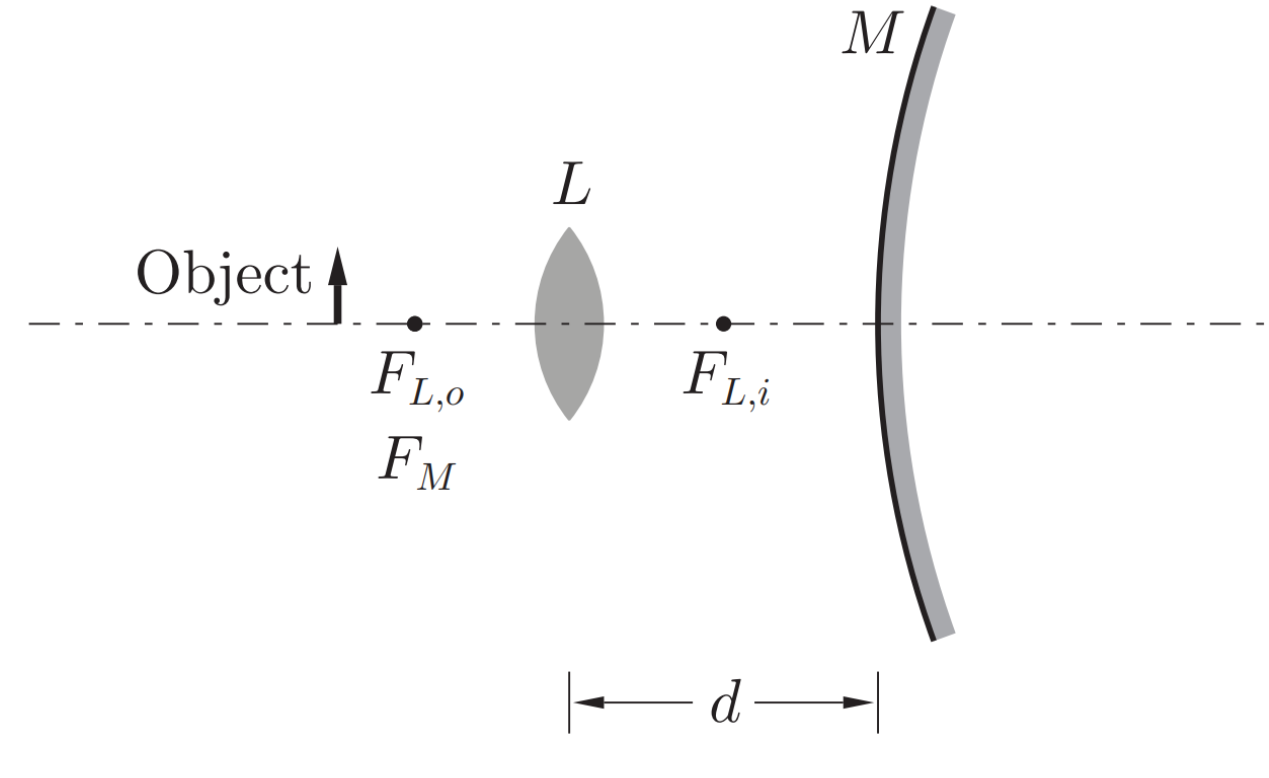
\includegraphics[width=0.68\linewidth]{Imágenes/tutorias/imagen_2023-10-12_145443062.png}
    \end{figure}
\end{multicols}

\item 
\begin{multicols}{2}
 Dos antenas de radio separadas 300 m transmiten simultáneamente señales idénticas a la misma longitud de onda. El radio en un automóvil que se desplaza al norte recibe estas señales. \textbf{a)} Si el vehículo se encuentra en la posición del segundo máximo, ¿cuál es la longitud de onda de las señales? \textbf{b)} ¿Cuánto más lejos debe viajar el auto para encontrar el siguiente mínimo en recepción? (Nota: No utilice la aproximación de ángulo pequeño en este problema.)

    \columnbreak
    
    \begin{figure}[H]
        \centering
        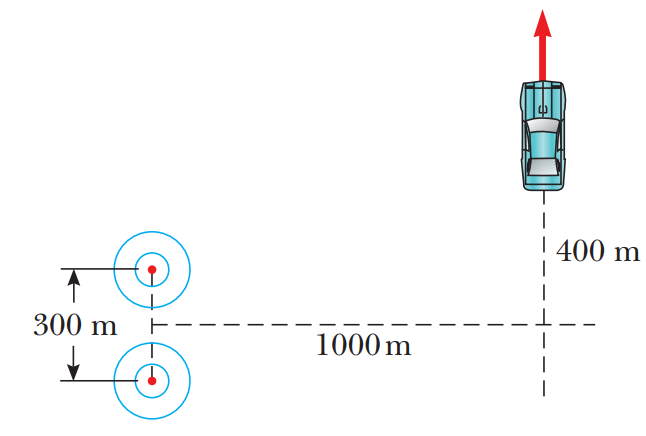
\includegraphics[width=0.75\linewidth]{Imágenes/clases/auto.png}
    \end{figure}
\end{multicols}

\item Considere que una lámina de plástico transparente, de índice de refracción $n$ y espesor $t$, se coloca entre la ranura superior y la pantalla con orientación tal que la luz pasa a través del plástico perpendicularmente a sus superficies, como se muestra en la figura:

\begin{multicols}{2}
    \begin{enumerate}
        \item Cuando se hace esto, el máximo central del patrón de interferencia se mueve hacia arriba en la pantalla en una distancia $y'$. Determine una expresión para la distancia $y'$ en términos de $d, L, N \text{ y } t$
    
        \item Ahora suponga que no se conoce el espesor de la lámina, pero sí se sabe que el rayo de luz tiene longitud de onda $\lambda$. Si el punto central de la pantalla es un punto oscuro en lugar de un punto brillante, ¿cuál es el grosor mínimo de la lámina de plástico?
    \end{enumerate}
    \columnbreak
    \begin{figure}[H]
        \centering
        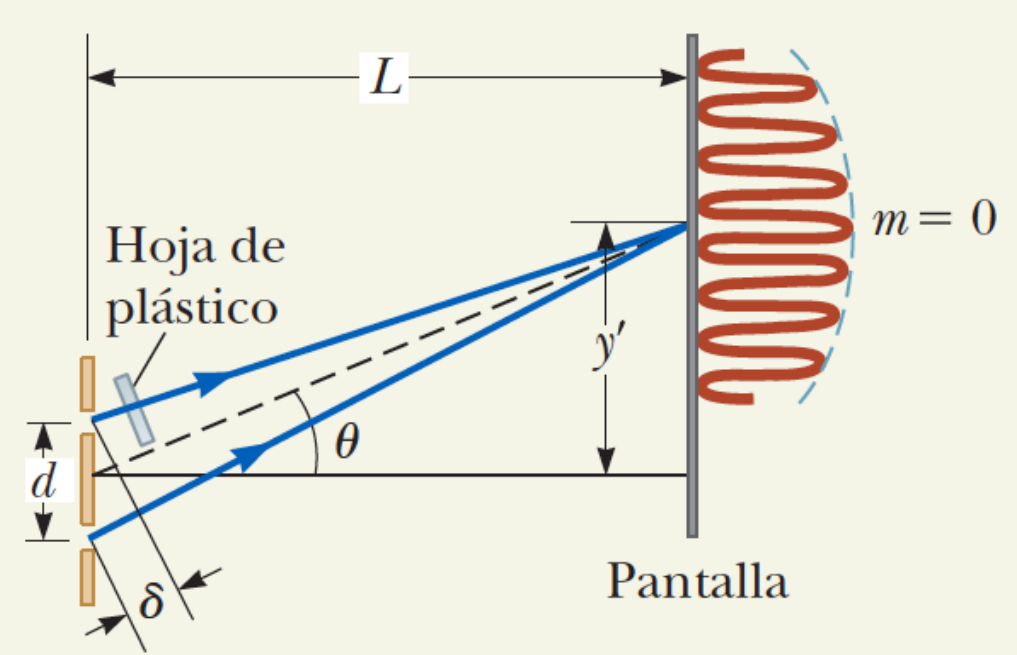
\includegraphics[width=0.9\linewidth]{Imágenes/tutorias/imagen_2023-10-12_144956321.png}
    \end{figure}
\end{multicols}

% Para imágenes vectoriales -> el texto tiene que estar en LaTeX
% \begin{figure}[htbp]
%   \centering
%   \svgpath{../Imagenes/ejercicios}  -> .. irse pa'trás 
%   \includesvg{ej5.svg}
% \end{figure}

\end{enumerate}
\end{document}
